% fig_mapping

\begin{figure}[!t]
\begin{center}

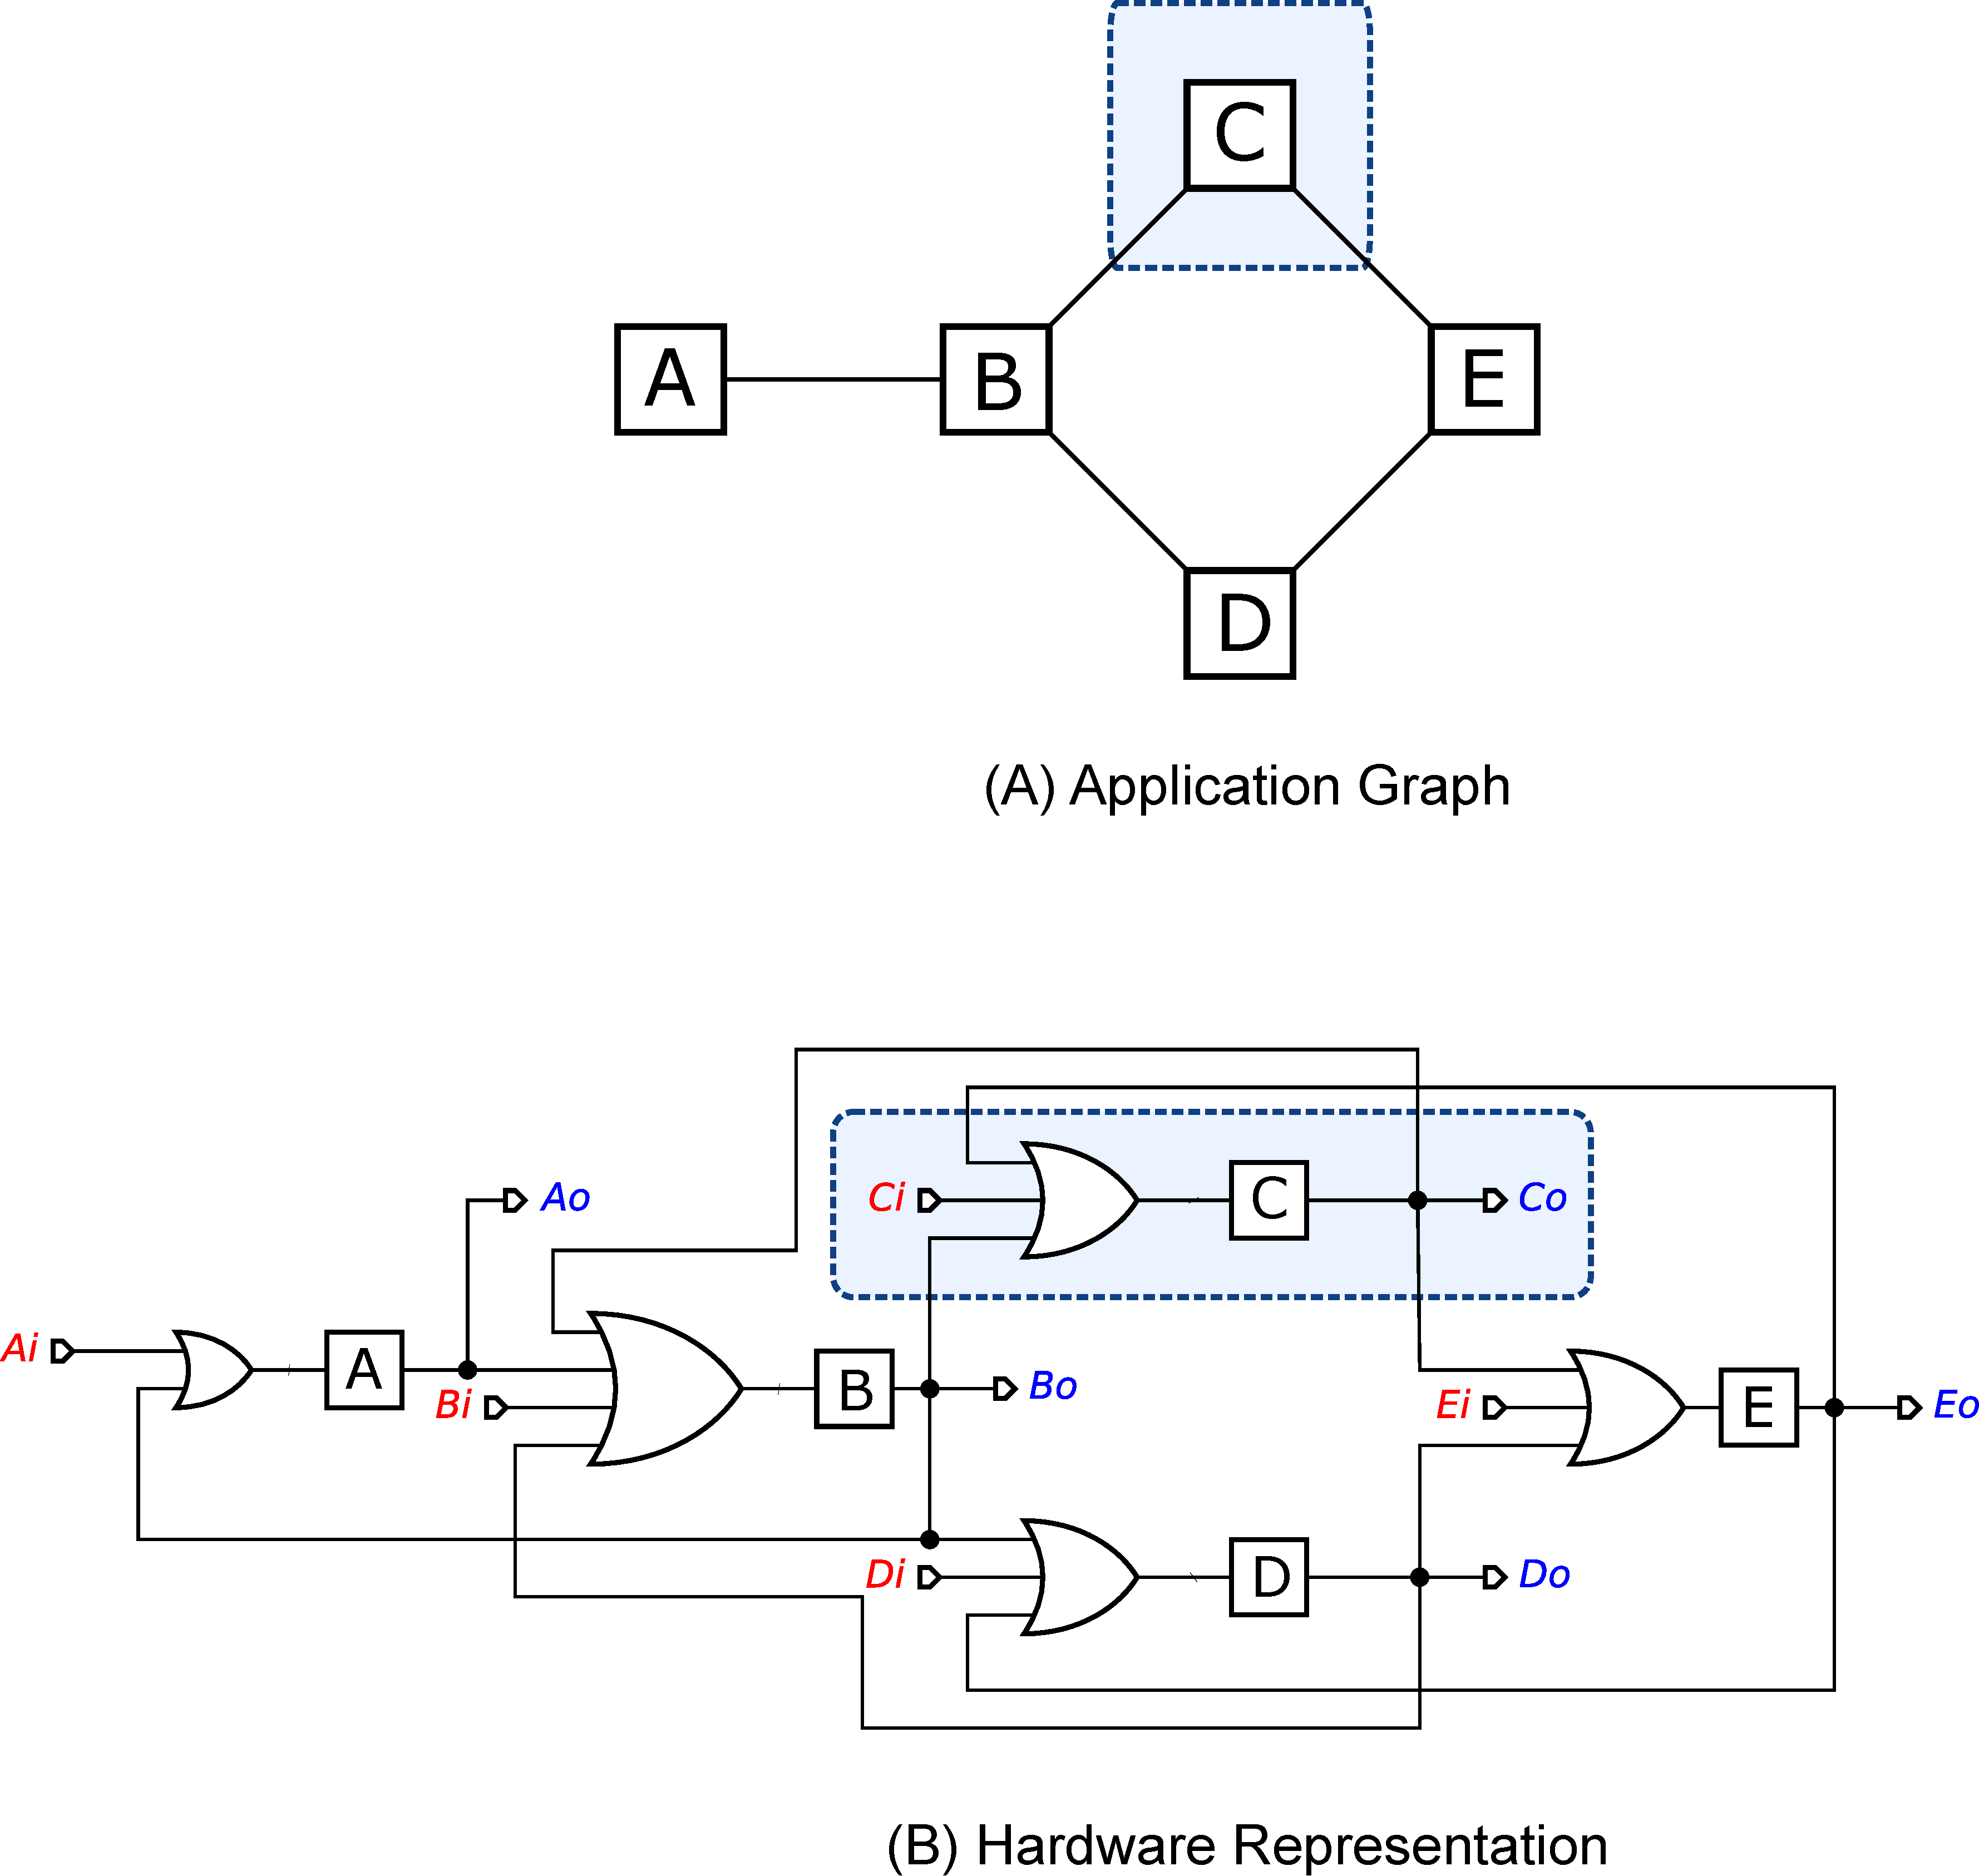
\includegraphics[width=8.8cm]{figures/fig_mapping}

\caption{
Mapping a network to hardware. Nodes are implemented as flip-flops, and edges as combinational paths.
Traversal is performed by propagating a logic high status between flip-flops, starting from a root node,
and completion is detected by monitoring the status of all nodes.
}

\label{fig_mapping}
\end{center}

\end{figure}
